\chapter{Interface Web}

Com arquitetura desenvolvida e disponível os seus utilizadores devem ter uma plataforma através da qual consigam acompanhar os registos provenientes da sua utilização da arquitetura. Esse é também um dos objetivos desta dissertação, ou seja, desenvolver uma interface através da qual cada utilizador consiga aceder aos seus dados e às várias informações relacionados com a monitorização efetuada através da solução desenvolvida. Serão apresentados neste capítulo a metodologia de desenvolvimento utilizada na conceção da interface web, os diferentes níveis de acesso existentes na plataforma, bem como as funcionalidades disponíveis para cada cada tipo de utilizador e ainda um conjunto de conclusões sobre a interface implementada.

\section{Padrão de Desenvolvimento}

No desenvolvimento da plataforma Web, através da qual os utilizadores poderão aceder aos seus registos de monitorização, o padrão de arquitetura de software utilizado foi o MVC. Este padrão, cuja sigla MVC signfica \textit{Model-View-Controller}, trata-se de um dos padrões de desenvolvimento de software mais utilizados atualmente, e tem por base promover a reutilização do código desenvolvido, bem como a separação de conceitos e definição de interação entre eles em termos de arquitetura de software\cite{bucanek2009model}. 

Este torna-se extremamente útil, e consequentemente bastante utilizado, com o aumento da complexidade das aplicações a desenvolver. Este facto levou a que existisse a necessidade de separar conceitos de forma a simplificar o processo de desenvolvimento para os responsáveis pela construção destas plataformas. Deste modo, torna-se fundamental a separação entre os dados da aplicação e a camada de apresentação, garantindo assim que as alterações feitas no \textit{layout} não interferem com a manipulação dos dados e que estes podem ser modificados sem que isso tenha repercussões no \textit{layout}. Esta separação apenas é possível pela existência de um componente responsável pela intermediação entre os dois, o controlador\cite{bucanek2009model}.

O modelo MVC, utilizado no desenvolvimento desta interface Web, divide assim os componentes da aplicação em três camadas: o \textit{Model} que representa os dados e o métodos de acesso e edição destes, a \textit{View} que corresponde à camada de visualização da aplicação, sendo a parte responsável pela iteração com os utilizadores. E por fim o \textit{Controller} que contém os métodos que processam os pedidos provenientes da \textit{View} e pode também invocar alterações no \textit{Model}, funcionando como um controlador da aplicação e a ponte entre as duas camadas restantes. Desta forma é possível organizar de forma mais modular a arquitetura de uma aplicação web, centrando em cada camada única e exclusivamente as funções para as quais essa foi concebida, simplificando estruturalmente o desenvolvimento da aplicação.

\section{Tipos de Acesso}

A interface web criada para complementar a utilização da arquitetura foi desenhada com dois níveis de acesso para os seus utilizadores. Desta forma, os dois tipos de perfis existentes terão permissão de acesso a diferentes funcionalidades e informações da plataforma. Esta divisão de permissões em apenas dois níveis baseia-se na necessidade de ter um acesso para o utilizador comum consultar as suas informações e registos, e outro acesso para que o administrador possa consultar todos os conteúdos de administração relevantes da plataforma.

O acesso com maior nível corresponde assim às permissões de administração. Este nível de acesso disponibiliza um conjunto alargado de informações sobre os utilizadores da arquitetura, dos registos de monitorização efetuados e ainda sobre os sensores conectados à arquitetura bem como o seu funcionamento. Este perfil de utilizador corresponde ao tipo de acesso mais elevado definido para esta interface e apenas um conjunto restrito de utilizadores devem ter acesso a estes conteúdos.

 \begin{figure}[htb]
   \centering
   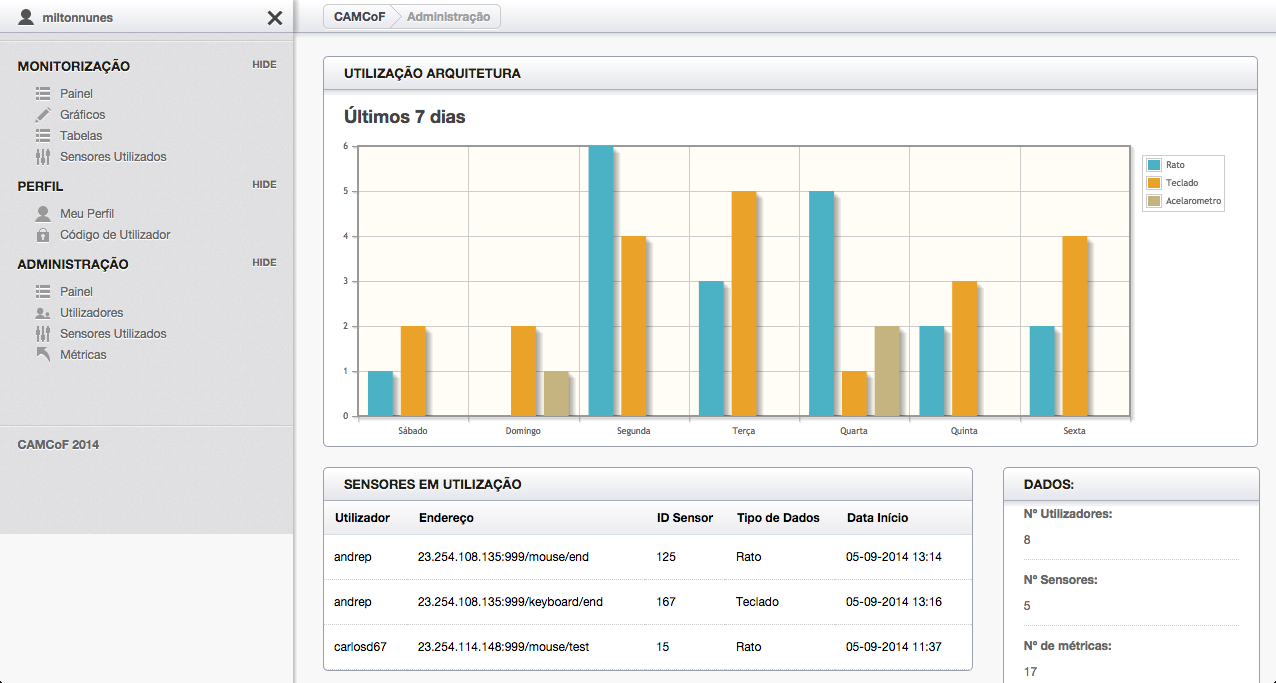
\includegraphics[scale=0.29]{Images/panel1.png}
   \caption{Página principal de Administrador}
\end{figure}

O outro nível de acesso implementado corresponde ao acesso atribuído aos utilizadores comuns da arquitetura. Através do seu acesso à interface os utilizadores da arquitetura conseguem aceder às suas informações pessoais e a todos os dados relacionados com a sua monitorização. Deste modo, tem acesso a todos os seus registos de monitorização apresentados de diferentes formas e pode ainda efetuar consultas sobre todo o seu histórico. Este nível representa um acesso mais restrito que o anterior, visto que limita os dados apresentados apenas aos correspondentes ao próprio utilizador e aos seus registos de monitorização.

 \begin{figure}[htb]
   \centering
   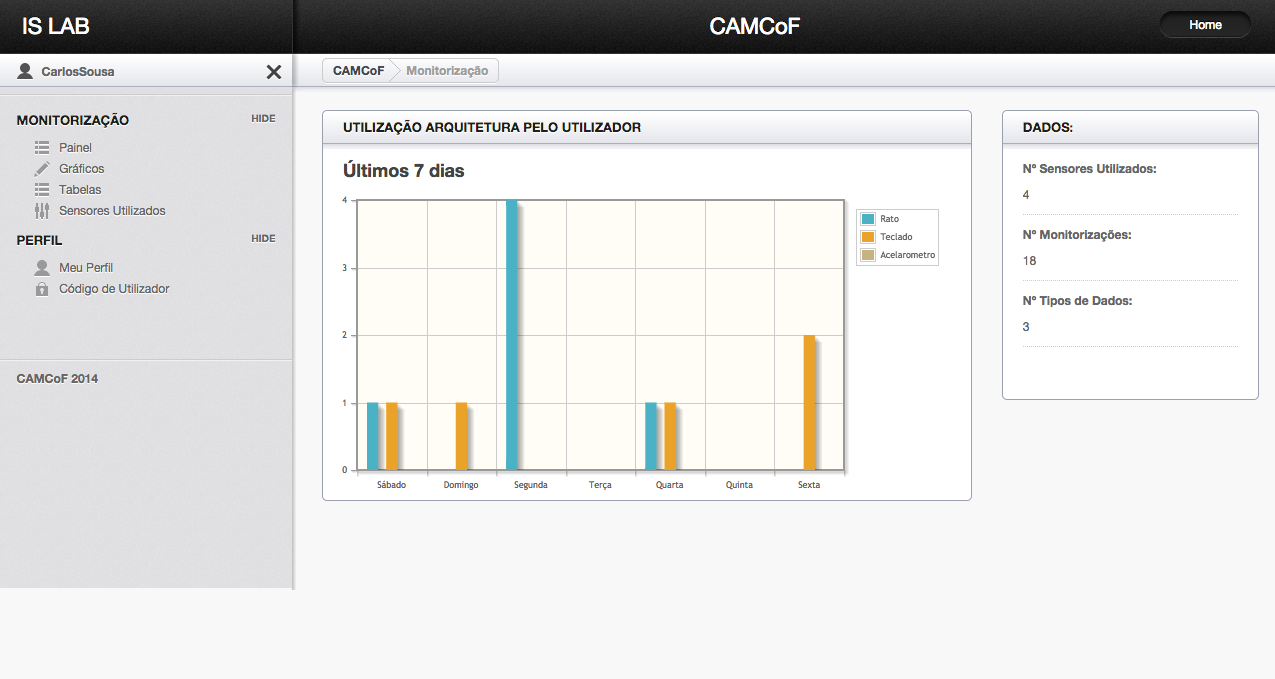
\includegraphics[scale=0.29]{Images/home1.png}
   \caption{Página principal de Utilizador}
\end{figure}

\section{Funcionalidades de Utilizador}

No contexto de utilização da arquitetura por parte de um utilizador, é extremamente importante este poder consultar e analisar os resultados da sua monitorização. Deste modo, um dos objetivos no desenvolvimento da interface foi fornecer aos utilizadores acesso a todo o seu histórico de registos provenientes da utilização da arquitetura desenvolvida. Cada utilizador terá assim na sua área pessoal acesso total a todo o conteúdo de informação recolhida e processada pela arquitetura. Para além disso terá ainda disponível diferentes formas de acesso e apresentação da informação, com o intuito de que os seus utilizadores possam tirar o máximo de proveito dos seus próprios dados.

Assim para além das informações mais genéricas apresentados a cada utilizador na sua página principal, este poderá aceder a duas áreas da interface nas quais poderá consultar todos os seus registos de monitorização. A diferenças entre estas duas áreas reside na forma de apresentação da informação. Na primeira área o utilizador poderá aceder aos seus registos sob a forma de tabela, selecionando o tipo de dados que pretende consultar e uma métrica associada ao tipo de dado escolhido. No caso de esse tipo de dados não conter nenhuma métrica disponível na arquitetura a informação será apresentada em bruto, tal como foi recolhida pelo dispositivo responsável pela monitorização. Para além disso, o utilizador poderá ainda escolher o período de monitorização que pretende, tendo em conta obviamente os dois parâmetros já definidos.

 \begin{figure}[htb]
   \centering
   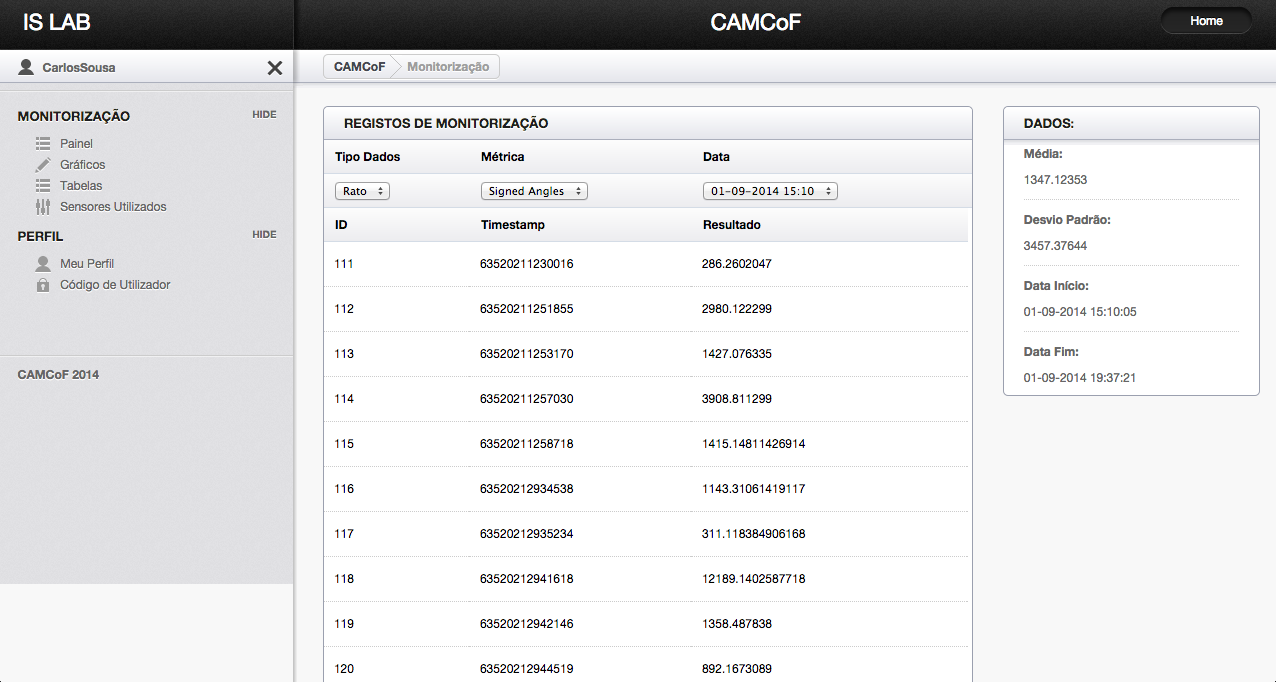
\includegraphics[scale=0.29]{Images/tables1.png}
   \caption{Página de visualização de registos de monitorização sob a forma de tabelas}
\end{figure}

A segunda área de apresentação dos registos de monitorização disponibilizada trata-se da apresentação de resultados através de gráficos. Esta forma de apresentação é bastante útil para os utilizadores pois permitem-lhe ter uma noção gráfica mais clara dos seus registos e variações comportamentais ao longo do período de monitorização. Esta área oferece assim uma forma mais simples de visualização e interpretação dos resultados. Tal como na área composta por tabelas, o utilizador poderá selecionar o tipo de dados, uma métrica associada e a data do período a visualizar. Neste caso em particular apenas os tipos de dados com métricas associadas serão apresentados devido à dificuldade em gerar gráficos através de informação em bruto.

 \begin{figure}[htb]
   \centering
   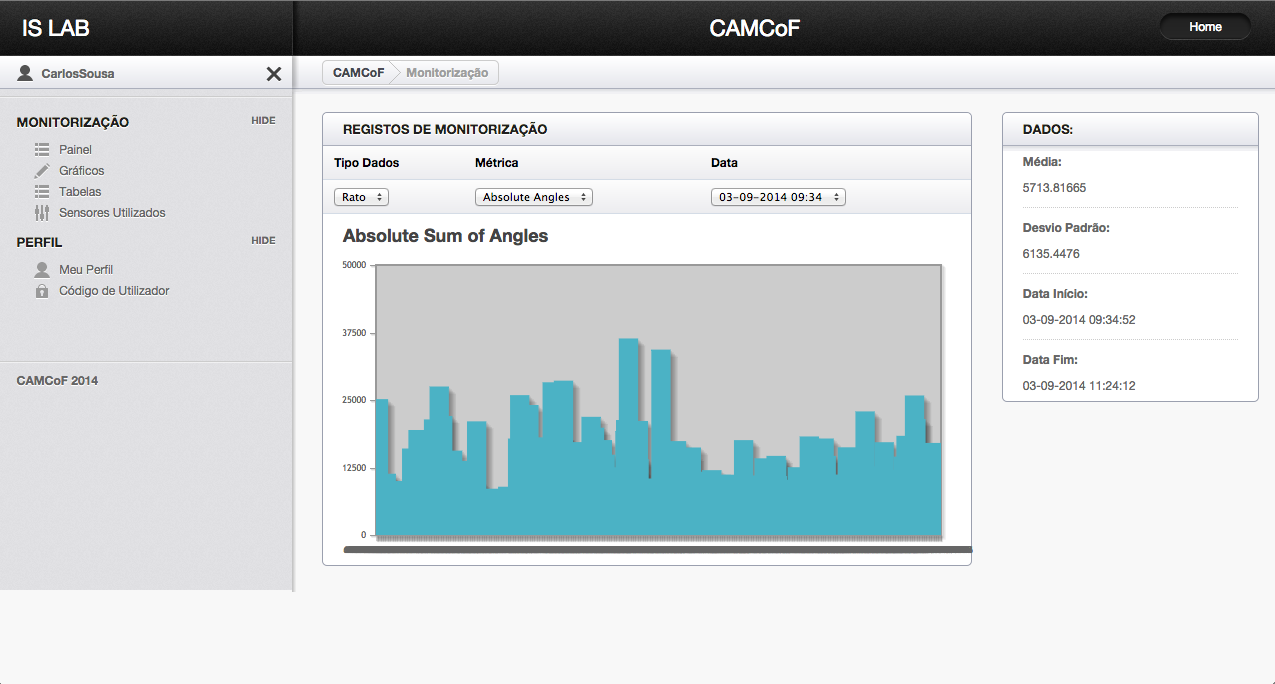
\includegraphics[scale=0.29]{Images/graphs1.png}
   \caption{Página de visualização de registos de monitorização sob a forma de gráficos}
\end{figure}


\section{Funcionalidades de Administração}

Relativamente às funcionalidades de administração, estas residem sobretudo no acesso a informação privilegiada. Tem como principal objetivo acompanhar a utilização da arquitetura e poder aceder a informações relativas a essa utilização. Desta forma, para além dos dados estatísticos apresentados no painel de administração, no qual pode, por exemplo, saber que utilizadores estão a ser monitorizados e quais os sensores utilizados no momento, o administrador tem acesso a outros conteúdos relevantes.

\begin{figure}[htb]
   \centering
   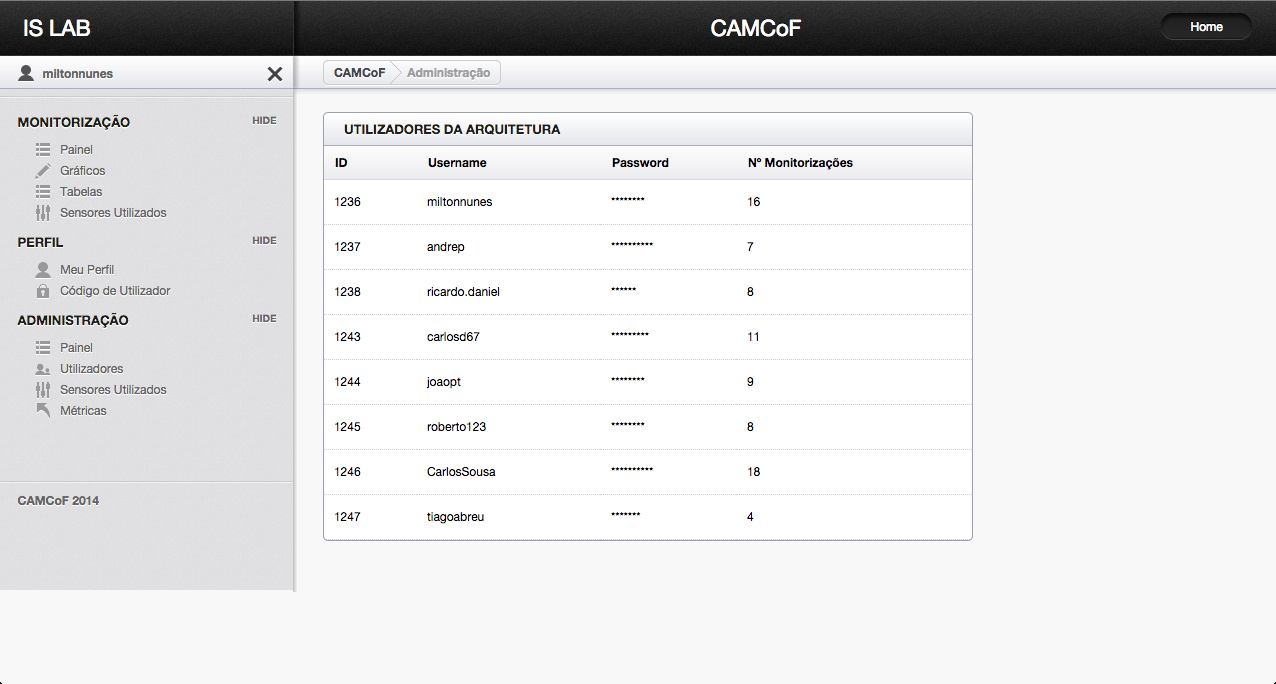
\includegraphics[scale=0.29]{Images/users1.png}
   \caption{Página de consulta de utilizadores da arquitetura}
\end{figure}

Cada administrador do sistema poderá consultar os dados de todos os utilizadores do sistema, podendo ver não só os seus dados, como também saber o número de monitorizações efetuado por cada um. Para além das informações relativas a utilizadores da arquitetura, o administrador tem também acesso aos registos dos sensores utilizados na arquitetura, independentemente do momento da sua utilização e ainda à lista de todas as métricas integradas na arquitetura. Todo este conjunto de funcionalidades permite a cada administrador acompanhar a utilização da arquitetura e aceder aos seus dados principais.

\begin{figure}[htb]
   \centering
   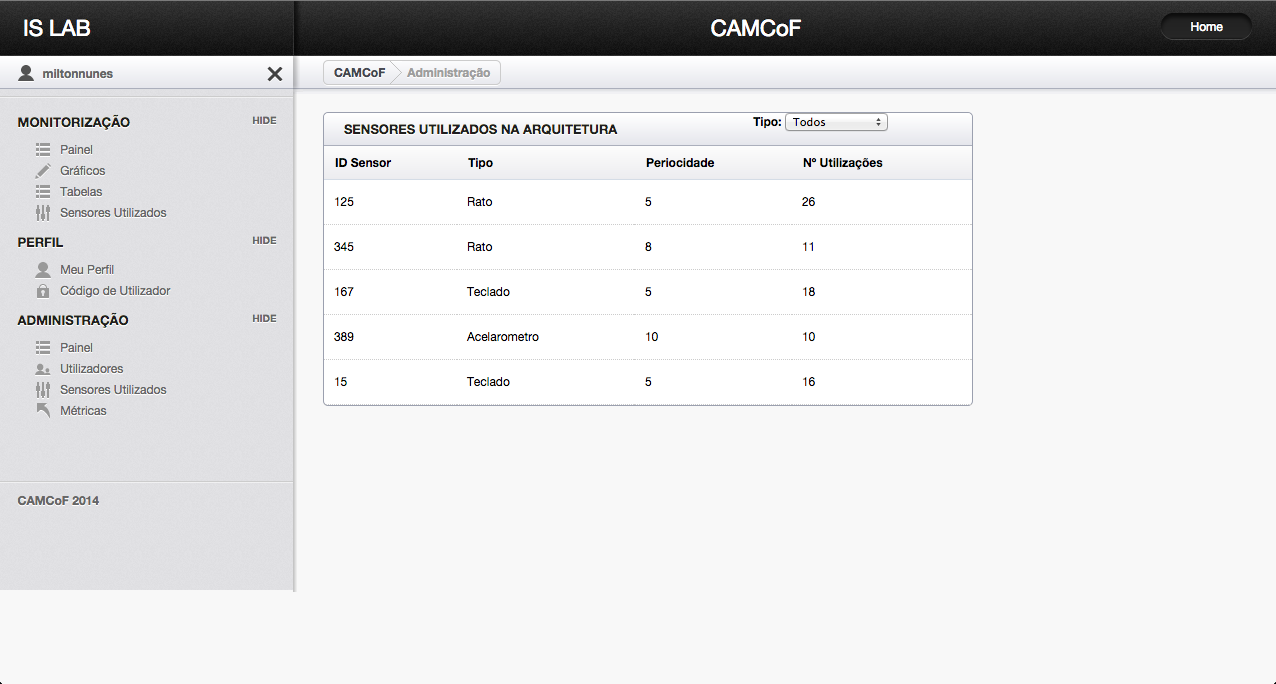
\includegraphics[scale=0.29]{Images/sensores1.png}
   \caption{Página de consulta de sensores registados na arquitetura}
\end{figure}


\section{Conclusão}

O padrão MVC utilizado no desenvolvimento desta plataforma revelou-se bastante útil e contribuiu para que a implementação da interface fosse um processo mais rápido do que seria expectável. A separação de componentes da aplicação e tratamento de cada função em específico na respetiva camada contribui para a simplificação do desenvolvimento da interface e consequentemente tornou o processo mais rápido e intuitivo. Apesar de não se tratar de uma aplicação com elevada complexidade, o potencial e capacidade deste padrão ficou bem patente no processo de desenvolvimento e demonstrou o porquê da utilização massiva deste padrão atualmente.

Quanto à interface construída, esta será certamente de grande utilidade não só para os utilizadores da arquitetura, como também para os administradores da aplicação. O objetivo consistiu em abranger ao máximo a arquitetura e a sua informação, não só resultante da monitorização mas também toda a que está diretamente relacionada com isso e com o funcionamento da arquitetura. Objetivo esse que se pode afirmar ter sido alcançado, sendo possível aos seus utilizadores aceder aos dados mais relevantes da arquitetura, consoante o seu nível de acesso na interface.

No caso concreto da apresentação dos dados relativos à monitorização e estatísticas diretamente relacionadas, estas foram implementadas da forma idealizada. Os dados estatísticos presentes nas páginas principais de cada tipo de utilizador dão pequenas, mas importantes, informações sobre a utilização da arquitetura, tanto relativamente ao utilizador em questão como à utilização efetuada por todos os utilizadores. Quanto às formas de apresentação dos resultados de monitorização foram desenvolvidas com o intuito de permitir ao utilizador aceder de forma mais genérica e de fácil interpretação aos registos através dos gráficos. No caso do utilizador pretender um acesso e análise mais pormenorizada poderá fazê-lo através das tabelas de registos. Todas estas funcionalidades foram implementadas com o intuito de permitir um acesso simples e prático a este conjunto de dados fundamentais.

Deste modo pode-se concluir que a interface criada é um importante complemento à arquitetura e às suas funcionalidades e uma ferramenta extremamente útil para os seus utilizadores. Tendo por base uma arquitetura que permite a recolha de diferentes tipos de informação, de forma distribuída, e o seu tratamento e agregação, era importante a existência de uma ferramenta que permitisse a consulta dos dados resultantes. Através da interface desenvolvida os utilizadores da arquitetura podem assim consultar de forma simples e intuitiva o resultado das suas monitorizações e informação relacionada. Esta interface web permite também comprovar a funcionalidade da arquitetura e verificar a sua capacidade de recolha e gestão da informação.

